\documentclass{article}

\usepackage[margin=1in]{geometry}
\usepackage{parskip}
\usepackage{datetime}
\usepackage{url}
\usepackage{hyperref}
\usepackage[utf8]{inputenc}
\usepackage{graphicx}
\usepackage{listings}

\lstset{
    basicstyle=\ttfamily
}

\newdateformat{required}{\twodigit{\THEMONTH}/\twodigit{\THEDAY}/\THEYEAR}
\raggedbottom

\begin{document}

\begin{titlepage}
    \begin{center}
        \begin{huge}
        House in Your Head \\[1cm]
        Team G1-FrigidWaters \\[2.2cm]
        { \bfseries System Design Specification } \\[1cm]
        Cycle \# 1\\[2.2cm]
        Date: \required\today\\[1cm]
        \end{huge}
    \end{center}
    \null \vfill
    \begin{large}
        Team Members: \\[0.5cm]
        Name: Samuel Bever\\[0.5cm]
        Name: Michael Conway\\[0.5cm]
        Name: Joseph Muoio\\[0.5cm]
        Name: Kyle Patron\\[0.5cm]
        Name: Kevin Zakszewski
    \end{large}
\end{titlepage}
\section*{\centering Table of Contents}
\makeatletter
\@starttoc{toc}
\newcommand{\hsubsubsection}{
\@startsection{subsubsection}{3}{\z@}%
                                     {-3.25ex\@plus -1ex \@minus -.2ex}%
                                     {-1.5ex \@plus -.2ex}% Formerly 1.5ex \@plus .2ex
                                     {R\normalfont\normalsize}}
\newcommand{\hparagraph}{
\@startsection{paragraph}{4}{\z@}%
                                     {-3.25ex\@plus -1ex \@minus -.2ex}%
                                     {-1.5ex \@plus -.2ex}% Formerly 1.5ex \@plus .2ex
                                     {R\normalfont\normalsize}}
\newcommand{\hsubparagraph}{
\@startsection{subparagraph}{5}{\z@}%
                                     {-3.25ex\@plus -1ex \@minus -.2ex}%
                                     {-1.5ex \@plus -.2ex}% Formerly 1.5ex \@plus .2ex
                                     {R\normalfont\normalsize}}
\setcounter{secnumdepth}{5}
\makeatother
\newpage
 

\section{Introduction}

\subsection{Purpose}
The purpose of this document is to describe the data, interface, architectural, and component-level design for our project. The architectural section will go over the modules and components, their relationship, and will describe the structure of the system as a whole. The interface section contains more detail on the system's user interface, data interface,  and the programming interface. Finally, in the remaining portion of this document, any other design details or relationships will be layed out .

\subsection{Scope}

This system is intended to be a Brain Computer Interface that will act as a bridge between data received from the Emotiv device and a home automation system. The Emotiv device and the home automation system are black boxes. We are more concerned with taking the data from the Emotiv device, interpreting it correctly and triggering the correct actions in the home automation system. Changing the functionality of the other two systems are out of the scope of this project. 

\subsection{Definitions, Acronyms, and Abbreviations}
\begin{description}
    \item[EEG] Can refer to:
        \begin{itemize}
            \item Electroencephalography - Recording of the brain's electrical
                activity 
	        \item Electroencephalogram - The device that is used to record the
	            brain's electrical activity

        \end{itemize}
    \item[Emotiv] The electroencephalogram hardware device, created by Emotiv
        Limited, used to read the user's brain activity (EEG)
    \item[Brain Computer Interface (BCI)] The class of devices that the Emotiv
        belongs to
    \item[Amyotrophic Lateral Sclerosis (ALS)] A neurodegenerative disorder
        that our target users suffer from. The main characteristics of ALS
        that we are concerned with in the scope of this project are the
        limited movement and mobility to complete paralysis.
    \item[API] software level functions which allow other parts of the system (or external systems) to interact and share data.
\end{description}


\subsection{Overview}

Section 2 discusses ...

\subsection{Requirements Traceability Matrix}
This section maps the relationship between requirement statements and detailed design entities.  As such it shows how requirements are covered by the design, and demonstrates the purpose for which design entity exists.
The values in the cells of the table show which requirements provide the purpose for each entity. The cell values are:

Blank – the design entity does not implement any of that requirement
P for Primary - the design entity implements all or most of the requirement
S for Secondary – the design entity implements a smaller but essential part of the requirement

\begin{tabular}{ | l | l |}

\end{tabular}

\newpage

\section{Architectural Description}

\subsection{External Interfaces}

We will only have two software interfaces that we will need to conform to. The
first is the input interface. For this we will have to use the pre-made
drivers to access the EEG. This confines our project to machines running a
relatively modern version of Windows, since the driver is not available for
any other operating system. The second interface that we have to conform to is
that of the home automation system.

The UI will consist of a binary tree of possibilities. At any one time only
one node is being displayed to the user and one of the two child nodes is
being selected to recursively repeat this process on. Leaf nodes will result
in actions, such as turning on the lights in a particular room. Which leaf is
selected will be based on the input of the EEG.

This section gives a description of the hardware and software interfaces. Also included is a basic prototype of the UI.

\subsection{Overview of modules / components}

\begin{figure}[h!]
	
  \centering
    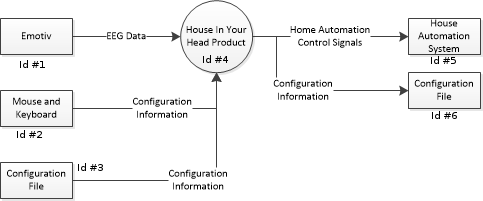
\includegraphics[width=0.7\textwidth]{DFD1}
   \caption{High level DFD}
   \label{fig:dfd1}
\end{figure}

\begin{figure}[h!]
	
  \centering
    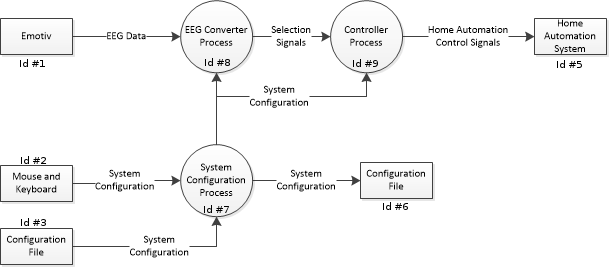
\includegraphics[width=0.7\textwidth]{DFD2}
   \caption{High level DFD with the main process broken out}
   \label{fig:dfd2}
\end{figure}

% TODO probably change this
\autoref{fig:dfd1} indicates the four external systems that
provide data to or accept data from our product. Three of these are trivial.
These are Id 2, Id 3, and Id 6. We accept input from the mouse and keyboard in
order to configure our system and we store the resulting configuration,
locally or externally as seems appropriate at the time. Apart from these, our
system accepts data from the Emotiv device through their driver and output
controlling signals to the home automation system.

\autoref{fig:dfd2} is a broken-out version of \autoref{fig:dfd1}. The System
Configuration Process (Id 7) must deal with system configuration. This
involves reading it (from an external source if necessary), modifying it,
writing it back for later use and providing it to the other parts of the
program. The EEG converter process (Id 8) takes in the EEG data and is
responsible for getting a clear signal out of it. The Controller process (Id
9) is responsible for storing the current state of the system, transitioning
states when appropriate and sending signals to the home automation system that
match the state.

\subsection{Structure and relationships}

\subsubsection{Component ID 1}
This component is the brain computer interface that provides an EEG signal into our system to control it.

\subsubsection{Component ID 2}
This is a mouse and keyboard. While this is not usually explicitly included, since we are using a BCI for most controls, we thought that it would be helpful.

\subsubsection{Component ID 3}
This is the source of the current configuration. This may be stored locally, or may be stored externally.

\subsubsection{Component ID 4}
This represents the totality of our product. It performs every action and completely controls the house given the EEG as input.

\subsubsection{Component ID 5}
This is the home automation system. When it receives signals, it changes a physical property of the house, such as whether a light is on or off, or what channel a stereo is tuned to.

\subsubsection{Component ID 6}
This is the configuration file again. It is identical to Id 3 except it is being written to instead of read from.

\subsubsection{Component ID 7}
This is the process that is in charge of managing the system configuration. It reads in the configuration, process is, modifies it if necessary, makes it available to the rest of the system, and writes it back if modified.

\subsubsection{Component ID 8}
This is the process responsible for converting the large amount of data of the EEG into a more understandable signal. This will consist of only one bit at any given time.

\subsubsection{Component ID 9}
This component translates the control signals generated into Id 8 and uses them to control the house. It does this by storing the current state of the system and then transitioning when it receives the proper signals from Id 8.
\newpage

\section{Interface Description}

\subsection{User Interface}



The user interface of the system is a rather simple one because most of the data we will receive and the choices the user will make are binary. There will be one type of screen where the user will cycle through the options of the objects that they can interact with in the home automation system. This is also the screen where the user makes the decision which object they want to interact with. When an object is chosen, they will be directed to the second type of screen. The second type of screen that handles the changing of the state of the object the user selects. From this screen the user can either change the state or return to the previous screen (the first type where the users cycle through the options). These two types UI of screen will make up the majority of the system. These designs will be modified or extra user interface designs will be implemented as necessary. 

\begin{figure}[h!]
	
  \centering
    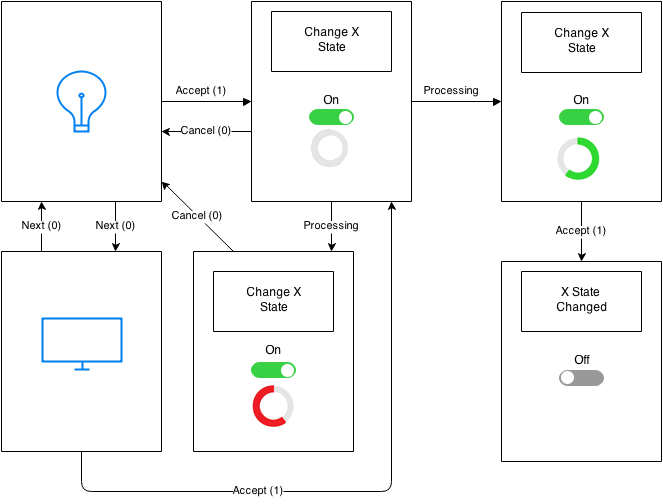
\includegraphics[width=0.7\textwidth]{UI_Mockup}
   \caption{Sample User interface}
   \label{fig:ui}
\end{figure}

\subsection{Data Interface}
\begin{figure}[h!]

  \centering
    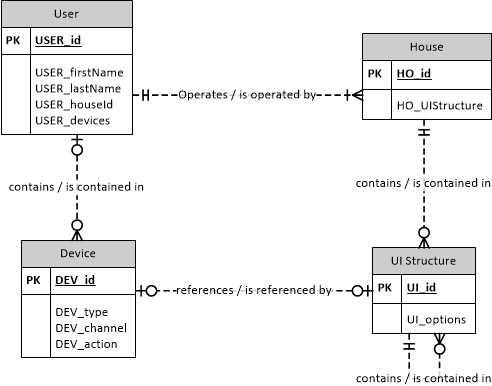
\includegraphics[width=0.5\textwidth]{ERD}
   \caption{ERD}
   	\label{fig:erd}
\end{figure}

The data flowing into our program will consist of a tuple of floats,
representing the EEG data at any given time. There will also be a JSON blob
that stores the parameters that should be used in signal extraction. The
output will be in the form of calling methods of the home automation system.
\autoref{fig:erd} shows the internal representation of the user, house and
state. This consists of a binary tree of UI structures, which may or may not
reference a device to call the method of.
% XXX Huh?

\subsection{Programming Interface} 
There is no need for a programming interface because it is a generic, self-contained system.

\newpage

\section{Detailed Design}

\subsection{Component Template Description}

\subsection{Design Entities}

\subsubsection*{1.0 - EEG Interpreter}
\begin{tabular}{ | l |  p{13.3cm} |}
\hline
\textbf{Type} & Module \\ \hline
\textbf{Purpose} & Determines if the current brain scan information matches the trained data \\ \hline
\textbf{Function} & Uses statistical techniques to look at the current EEG information coming from the user's brainwaves and compares this to the data that was trained to see if it matches one of the trained classes. \\ \hline
\textbf{Subordinates} & None \\ \hline
\textbf{Dependencies} & Relies on Training datastore (2.2). There needs to be trained models to compare the stream of data to. \\ \hline
\textbf{Interface} & The EEG Interpreter will have an API that can be polled by other components. \\ \hline
\textbf{Resources} & The EEG information comes from the emotive device. \\ \hline
\textbf{Processing} & Various statistical techniques will be explored. At first, a simple algorithm that checks whether the EEG information falls within a given threshold to the training data, but more advanced techniques will be explored as well. \\ \hline
\textbf{Data} & See ERD in Section 3 \\ \hline
\end{tabular}

\subsubsection*{2.0 - Training Module}
\begin{tabular}{ | l |  p{13.3cm} |}
\hline
\textbf{Type} & Module \\ \hline
\textbf{Purpose} & Trains a model for the current user for each state. \\ \hline
\textbf{Function} & Delegates to state trainers for each state that needs to be trained for the current user. Then stores this in the Training Datastore (2.2). \\ \hline
\textbf{Subordinates} & State Trainer (2.1). Every state that needs to be trained will be trained through a specific state trainer for that state. \\ \hline
\textbf{Dependencies} & Training Datastore (2.2). This is needed to save the trained models. \\ \hline
\textbf{Interface} & None \\ \hline
\textbf{Resources} & None \\ \hline
\textbf{Processing} & For each State Trainer (2.1) that is untrained, train the state model for that trainer. Then, save the results to the Training Datastore (2.2). \\ \hline
\textbf{Data} & See ERD in Section 3 \\ \hline
\end{tabular}

\subsubsection*{2.1 - State Trainer}
\begin{tabular}{ | l |  p{13.3cm} |}
\hline
\textbf{Type} & Module \\ \hline
\textbf{Purpose} & Trains a model for a single state. \\ \hline
\textbf{Function} & Trains a model for a specific state. Each state trainer trains on one state, so there will be a State Trainer for the resting state, active state, and any other states deemed necessary in the future. \\ \hline
\textbf{Subordinates} & None \\ \hline
\textbf{Dependencies} & GUI Module (3.0). To train a model, interaction with the user of the system is required. This is done through a Graphic User Interface.  \\ \hline
\textbf{Interface} & None \\ \hline
\textbf{Resources} & None \\ \hline
\textbf{Processing} & Interact with the user on the screen until a model is built based on the user's personal EEG. \\ \hline
\textbf{Data} & See ERD in Section 3 \\ \hline
\end{tabular}

\subsubsection*{2.2 - Training Datastore}
\begin{tabular}{ | l |  p{13.3cm} |}
\hline
\textbf{Type} & Data store \\ \hline
\textbf{Purpose} & Holds the trained data for the current user. \\ \hline
\textbf{Function} & Holds all the trained states for the current user of the system. This includes the resting state and the active state at a minimum. Other states will be explored in the future. \\ \hline
\textbf{Subordinates} & None \\ \hline
\textbf{Dependencies} & None \\ \hline
\textbf{Interface} & The training datastore will have an API that allows read and write access to it. \\ \hline
\textbf{Resources} & May need hard disk space if it will be saved permanently.  \\ \hline
\textbf{Processing} & The currently loaded user's data will be the only data retrieved. Loading from disk and saving to disk are allowed. \\ \hline
\textbf{Data} & See ERD in Section 3 \\ \hline
\end{tabular}

\subsubsection*{3.0 - GUI Module}
\begin{tabular}{ | l |  p{13.3cm} |}
\hline
\textbf{Type} & Module \\ \hline
\textbf{Purpose} & Hands output from the system to an external monitor. \\ \hline
\textbf{Function} & All interaction with the user is through an external monitor. This system handles all output to the screen. \\ \hline
\textbf{Subordinates} & None \\ \hline
\textbf{Dependencies} & None \\ \hline
\textbf{Interface} & There will be a writer API to allow other parts of the system to output to the screen. \\ \hline
\textbf{Resources} & External Monitor \\ \hline
\textbf{Processing} & The GUI module will wait until given something to write to the screen. When it is given a request, it will write that request to the screen. \\ \hline
\textbf{Data} & See ERD in Section 3 \\ \hline
\end{tabular}

\subsection*{4.0 - Home Automation Interface}
\begin{tabular}{ | l |  p{13.3cm} |}
\hline
\textbf{Type} & Module \\ \hline
\textbf{Purpose} & Interfaces with external home automation controls. \\ \hline
\textbf{Function} & Manages the system's interface with external home
automation controls. This includes providing the rest of the system with
information about available controls, maintaining any necessary state, and
processing requests to manipulate the home via the controls. \\ \hline
\textbf{Subordinates} & None \\ \hline
\textbf{Dependencies} & None \\ \hline
\textbf{Interface} & The interface will support querying for information about
available home controls and to manipulate the home via the controls. \\ \hline
\textbf{Resources} & Home automation system controls \\ \hline
\textbf{Processing} & The module will query control state as necessary and
reject requests that are not valid in the current state. \\ \hline
\textbf{Data} & See ERD in Section 3 \\ \hline
\end{tabular}

\newpage

\section{Reuse and Relationships to other Products}
\label{sec:ReuseRel}

There has been previous related work done with the Emotiv device by related
researchers. However, their interface was unappealing and their code messy. It
may be referenced to help understand the Emotiv device, but it will not be
reused directly.

There are very few commercially available BCI devices, and often there is no
software available for them. The few that do exist are prohibitively
expensive. Having the Emotiv available at a reasonable price will improve the
quality of life for many ALS patients.

\newpage

\section{Design decisions and tradeoffs}

The first design decision that was made was what type of interface to use.
The options available were EEG sensor devices, eye movement trackers, and
facial muscle detecting devices. EEG sensors seemed the best fit as they
will work for all ALS patients, including those that are ``locked in.'' A
locked-in patient may be unable to use their facial muscles or move their
eyes. In addition, this means that a patient will not have to relearn how to
use the system with new interfaces as their disease progresses.

Another design decision was what device should be used to best assist ALS
patients. As noted in \autoref{sec:ReuseRel}, there already exist devices with
similar functionality, but they are much more expensive. The Emotiv is \$500,
which is affordable when compared to its alternatives. The Emotiv is capable
of detecting up to four thoughts plus a neutral state, which provides enough
flexibility to design features in a number of ways.

Given this flexiblity, deciding how users should interface with the system was
the next step. Previous user reviews indicated that training the Emotiv to
recognize multiple thoughts was challenging, suggesting that a binary
interface would be the most useful. On the other hand, an interface that uses
a larger substantial branching would enable users to navigate it much more
quickly. The binary interface was chosen in order to maximize ease-of-use.

% TODO Is this a design decision, or was it made as a part of requirements?
The main purpose of the interface, home automation, was decided upon because
it allows patients to regain capabilities that they have lost. It also
serves as a proof of concept for interfacing with nontrivial systems.

\newpage

\section{Psuedocode for components}

\subsection*{1.0 - EEG Interpreter}

% TODO Does this make any sense?

\begin{lstlisting}
repeat forever:
    monitor EEG
    if EEG in a trained state:
        notify all registered listeners
        % TODO OR call all registered callbacks
\end{lstlisting}

\subsection*{2.0 - Training Module}

Upon training request:

\begin{lstlisting}
for each untrained State Trainer:
    run the trainer
save results to Training Datastore
\end{lstlisting}

Each State Trainer:

\begin{lstlisting}
repeat until trained:
    display prompt
    collect data from EEG Interpreter
    update training parameters
\end{lstlisting}

\subsection*{3.0 - GUI Module}

Upon menu display request:
\begin{lstlisting}
% TODO OPTION A
display menu
for each menu option:
    register callback for corresponding state in EEG Interpreter
% TODO OPTION B
display menu
register self as EEG Interpreter listener for necessary states
upon state notification, perform action
\end{lstlisting}

\subsection*{4.0 - Home Automation Interface}

Upon receiving a control request:

\begin{lstlisting}
if request is valid:
    perform action
else:
    report error
\end{lstlisting}

\newpage

\section{Appendicies}

% N/A?

\newpage

\section*{\centering Table of Contributions}
\begin{tabular}{| l | l | l | l |}
    \hline
     & Section & Writing & Editing \\
    \hline \hline
		1 & 2, 3.2 & Kyle Patron & \\ \hline
		2 & & Joe Muoio & \\ \hline
		3 & & Sam Bever & \\ \hline
		4 & & Michael Conway &  \\ \hline
		5 & & Kevin Zakszewski &  \\ \hline
\end{tabular}
\newpage
\noindent I certify that:
\begin{itemize}
\item This paper/project/exam is entirely my own work.
\item I have not quoted the words of any other person from a printed source or a website without indicating what has been quoted and providing an appropriate citation.
\item I have not submitted this paper / project to satisfy the requirements of any other course.
\end{itemize}

\vspace{1cm}
\noindent\makebox[\textwidth][l]{
Signature:
\makebox[5cm][l] {\underline{Samuel Bever}} 
\ \ Date:
\makebox[4cm][l] {\underline{\required\today}} 
}


\vspace{0.5cm}
\noindent\makebox[\textwidth][l]{
Signature:
\makebox[5cm][l] {\underline{Michael Conway}} 
\ \ Date:
\makebox[4cm][l] {\underline{\required\today}} 
}

\vspace{0.5cm}
\noindent\makebox[\textwidth][l]{
Signature:
\makebox[5cm][l] {\underline{Joe Muoio}} 
\ \ Date:
\makebox[4cm][l] {\underline{\required\today}} 
}

\vspace{0.5cm}
\noindent\makebox[\textwidth][l]{
Signature:
\makebox[5cm][l] {\underline{Kyle Patron}} 
\ \ Date:
\makebox[4cm][l] {\underline{\required\today}} 
}

\vspace{0.5cm}
\noindent\makebox[\textwidth][l]{
Signature:
\makebox[5cm][l] {\underline{Kevin Zakszewski}} 
\ \ Date:
\makebox[4cm][l] {\underline{\required\today}} 
}

\vspace{\fill}
\subsection*{Grading}
The grade is given on the basis of quality, clarity, presentation, completeness, and writing of each section in the report. This is the grade of the group. Individual grades will be assigned at the end of the term when peer reviews are collected.
\end{document}
